\documentclass[11pt,a4paper]{article}

\usepackage{titling, palatino, booktabs, graphicx}
\usepackage[margin=2cm]{geometry}
\usepackage[none]{hyphenat}
\usepackage{listings}

\usepackage{color}

\definecolor{dkgreen}{rgb}{0,0.6,0}
\definecolor{gray}{rgb}{0.5,0.5,0.5}
\definecolor{mauve}{rgb}{0.58,0,0.82}

\lstset{frame=tb,
  language=Java,
  aboveskip=1mm,
  belowskip=1mm,
  showstringspaces=false,
  columns=flexible,
  basicstyle={\small\ttfamily},
  numbers=none,
  numberstyle=\tiny\color{gray},
  keywordstyle=\color{blue},
  commentstyle=\color{dkgreen},
  stringstyle=\color{mauve},
  breaklines=true,
  breakatwhitespace=true,
  tabsize=3,
  escapeinside={||},
  mathescape=true
}

\begin{document}
\pagenumbering{gobble}
\setlength{\droptitle}{-5em}
\title{
Emerging Architecture Design\\ 
version 2.0
}
\date{\today}
\maketitle

\section{Introduction}
This document provides an overview of the architecture that is going to be built for this project. The components are covered from a high level view, to give a representation of how the different components work and the dependencies between them.

\subsection{Design goals}
The following design goals will be maintained throughout the project:
\begin{itemize}
\item
\textbf{Performance}\\
The game server will have to serve requests from  potentially a couple hundred players at any given moment. To minimize the amount of lag introduced by latency of networks, we have to design the system in such a way that the game experience seems fluent to the users. For this reason we will use non-blocking sockets to handle all requests in parallel and use an event-driven architecture.

\item
\textbf{Code reuse}\\
Dividing the different types of logic into modules is good for maintainability, but we will only get this advantage if logic that is similar for both components can be reused. To support this, we have divided the project into three sub-projects: \emph{Riverrush-Server}, \emph{Riverrush-Screen} and \emph{Core}. The \emph{Core} project contains all code shared between modules to maximize the possibility of reusing code. The modules with \emph{Riverrush-} in front of them are modules that can be run as applications.

\item
\textbf{Modularity} \\
As explained later, the game will involve three modules that work together. The modules are designed so they don't crash when one module fails. To support modularity, we will use the event-driven architecture to let the players update game state and also to let sub-components communicate.

\end{itemize}

\newpage

\section{Software architecture views}
This chapter is about architecture of the system. In the first paragraph the different parts of the system are explained and the relations between them. In the second paragraph the link between the software and the hardware are discussed. The third paragraph illustrates the data management of the system.

\subsection{Subsystem decomposition (sub-systems and dependencies between them)}
The system is broken down into 3 subsystems with a shared library to enable modularity. This way, all modules can be maintained separately while still being able to reuse shared code.\\
\\
The system uses a MVC pattern spread out over the modules. The Model and controller are located in the Server and the view is located in the Screen. The system also uses an observer pattern to make the game event-driven through the event dispatcher. 

\begin{itemize}
\item \textbf{Screen} \\
The screen code is located in the \emph{Riverrush-Screen} module. The screen connects to the server via a specialized protocol on top of WebSockets. Its role is to display the model changes on the screen. For this purpose the screen uses libGDX's graphical capabilities. The screen receives events about the current game state (a.k.a. Domain events) over the protocol from the server. These events are then processed and put into action on the screen.\\

\item \textbf{Client} \\
The client is a static HTML/JS website that is separate from the rest of the project. It is used to control the game from a smart phone or computer. It sends commands to the server over WebSockets when the user moves his/her phone. It also receives domain events back from the server to update the user screen accordingly with suitable information.\\
\\
The client uses an accelerometer to detect the user commands. If the accelerometer is not supported on the device the client falls back to swipe gestures.

\item \textbf{Server} \\
The server code is located in the \emph{Riverrush-Server} module. The server runs the game engine and holds the model of the game in memory. Domain events are used to notify the connecting clients if there is any relevant change to the state of the game. The server hosts separate endpoints to serve users and to connect the screen. This creates opportunity for socket-level optimization between the server and the screen because these modules are not required to use WebSockets for communication. We have chosen for this set-up because the connection between the server and the screen is likely to become a performance bottleneck. It also leaves the possibility to run the server in a cloud environment, which would cut the hardware costs of the game dramatically.\\
\\
The server is setup in a way that allows for great adaptability. When a client sends a join event to the server it creates a virtual user in the game engine that is coupled to an entity in the game. This virtual user is coupled to the specific web socket of that client. Through this setup the virtual user can be easily swapped out for a virtual user controlled by an AI (Artificial Intelligence) or some sort of hardware input system, like keyboard controls.\\
\\
All communications between the virtual user and the domain model (The model containing all the game state) goes through the event dispatcher. Commands from the client are given to the event dispatcher and executed by the command handlers on the domain model. When the domain model wants to notify other systems, it can send a domain event through the event dispatcher and any part of the game can listen to it and act upon it.\\
\\
The game state is handled by the state pattern that is built in the game. Each event that is fired on the game is first routed through the game states so it can determine if it is allowed to process the event. There are two places where this happens: 
\begin{itemize}
\item 
The game state where the system checks if the game is in a certain state like playing game state
\item
The animal state where the system checks if the animal is \emph{on the boat} / \emph{in the air} or \emph{in the water}.
\end{itemize}

\item \textbf{Core library} \\
The core code is located in the \emph{Core} module. The core contains all classes that can be used by both the screen and the server. This involves for example:
\begin{itemize}
\item Protocol code to send and receive game events.
\item Event dispatching code. Both modules use events to communicate and update their internal state.
\item Game entity classes. Both modules need a compatible version of the data model, the server to apply game mechanics to them, and the screen uses entities for display.
\end{itemize}

\end{itemize}

\subsection{Hardware/software mapping}
Each module is backed by some hardware. In order to run the server and the screen, at least one machine is needed, This set-up will practically eliminate latency between the screen and the server, but it has to run on a more expensive machine to support high loads.\\
\\
Another set-up is to run the screen and the server on different machines. This allows for scenario's where the machine connected to the auditorium beamers does not support a high networking load. The server can be run on a machine with well performing network hardware and send only relevant events to the screen.\\
\\
A third option is to run the server in a cloud environment and offer a subscription-fee to auditoriums. This reduces upfront costs and eliminates the requirement of high-end hardware inside the auditorium itself.\\
\\
The client HTML/JS application runs on all smart phone browsers that support WebSockets. 
\\
\newpage

This is an overview of all the components:\\
\\
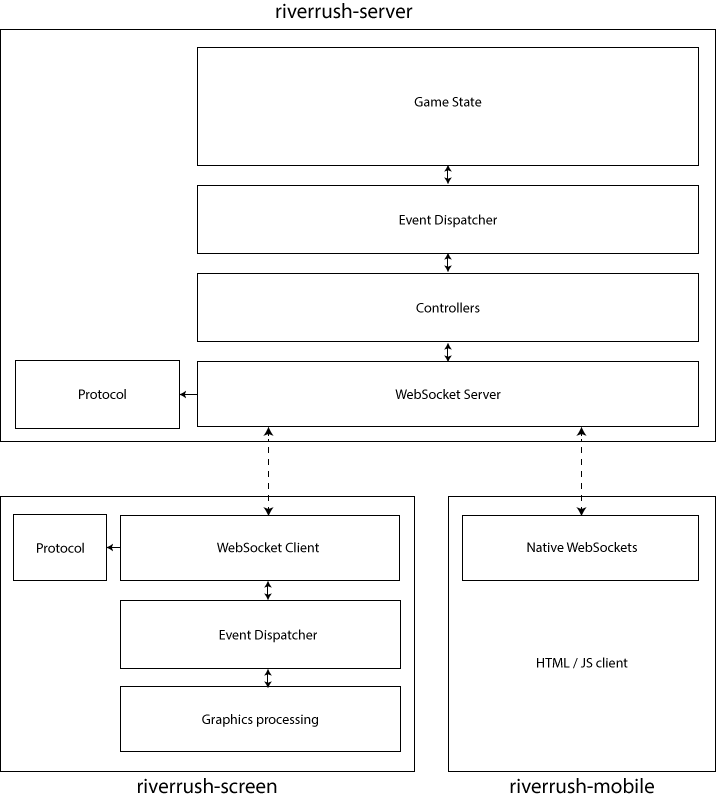
\includegraphics[scale=0.6]{arch.png}

\end{document}
